\usetikzlibrary{shapes.geometric, arrows}

\tikzstyle{process} = [rectangle, rounded corners, minimum width=3cm, minimum height=1cm, text centered, draw=black, fill=orange!30]
\tikzstyle{arrow} = [thick,->,>=stealth]

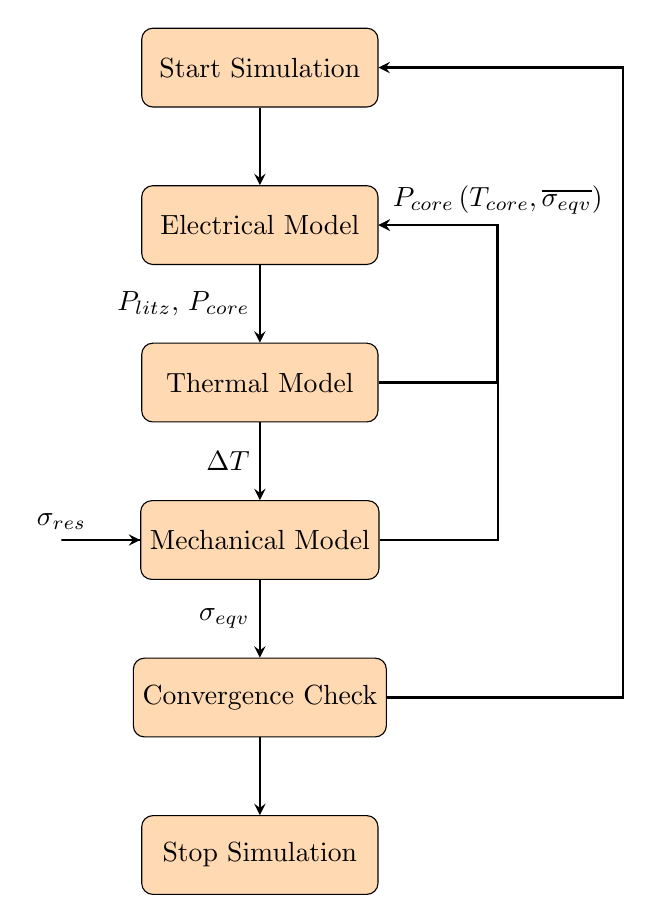
\begin{tikzpicture}[node distance=2cm]

% Nodes
\node (start) [process] {Start Simulation};
\node (electrical) [process, below of=start] {Electrical Model};
\node (thermal) [process, below of=electrical] {Thermal Model};
\node (mechanical) [process, below of=electrical, yshift=-2cm] {Mechanical Model};
\node (convergence) [process, below of=mechanical] {Convergence Check};
\node (stop) [process, below of=convergence] {Stop Simulation};

% Arrows
\draw [arrow] (start) -- (electrical);
\draw [arrow] (electrical) -- (thermal) node[midway,left] {$P_\text{litz}$, $P_\text{core}$};
\draw [arrow] (thermal) -- (mechanical) node[midway,left] {$\Delta T$};
\draw [arrow] (mechanical) -- (convergence) node[midway,left] {$\sigma_\text{eqv}$};
\draw [arrow] (convergence) -- (stop);
\draw [arrow] (mechanical.west) -| ++(-1,0) node[midway,above] {$\sigma_\text{res}$} -- (mechanical.west);
\draw [arrow] (mechanical.east) -- ++(1.5,0) |- (electrical.east) node[midway,above] {$P_\text{core}\left(T_\text{core}, \overline{\sigma_\text{eqv}}\right)$};
\draw [arrow] (thermal.east) -- ++(1.5,0) |- (electrical.east) node[midway,right] {};
\draw [arrow] (convergence.east) -- ++(3,0) |- (start.east) node[midway,right] {};

\end{tikzpicture}
